\documentclass[xetex,20pt]{scrartcl}
\usepackage{xltxtra,polyglossia}
\usepackage{pst-node,pspicture}
\usepackage{geometry}
\usepackage{array}

\setmainfont[Mapping=tex-text,Scale=1.0]{FreeSerif}
\setsansfont[Mapping=tex-text,Scale=1.0]{FreeSans}
\setmonofont{FreeMono}

\newfontfamily\hana{HAN NOM A}
\newfontfamily\hanb{HAN NOM B}
\newfontfamily\sil{Charis SIL}

\setmainlanguage[spelling=new]{german}
\setotherlanguage{english}

% set the new font width, declare the new lengths first
\newlength\MyWidth
\newlength\MyHeight
% set the new lengths
\setlength\MyWidth{12cm} % hier die Breite eintragen
\setlength\MyHeight{6.5cm} % hier die Höhe eintragen

% set new lengths to put the picture
\newlength\MyWput
\newlength\MyHput
\setlength\MyWput{\MyWidth}
\setlength\MyHput{\MyHeight}
% calculate the values by dividing etc.
\divide\MyWput by 2
\divide\MyHput by 2
\addtolength\MyHput{-\MyHeight}
\addtolength\MyHput{10 pt}
\makeatletter
\addtolength\MyHput{\@ptsize pt}
\makeatother

\geometry{papersize={\MyWidth,\MyHeight},total={\MyWidth,\MyHeight}}

\newcolumntype{x}[1]{%
>{\centering\hspace{0pt}}p{#1}}

\parindent 0pt
\begin{document}
\thispagestyle{empty}

\rput(\MyWput,\MyHput){%
\pspicture[showgrid=false](0,0)(\the\MyWidth,\the\MyHeight)
% Insert your Code here, as you like! Coordinate system starts with 0,0 on the left bottom of the
% page. 
\rput(6,3.24){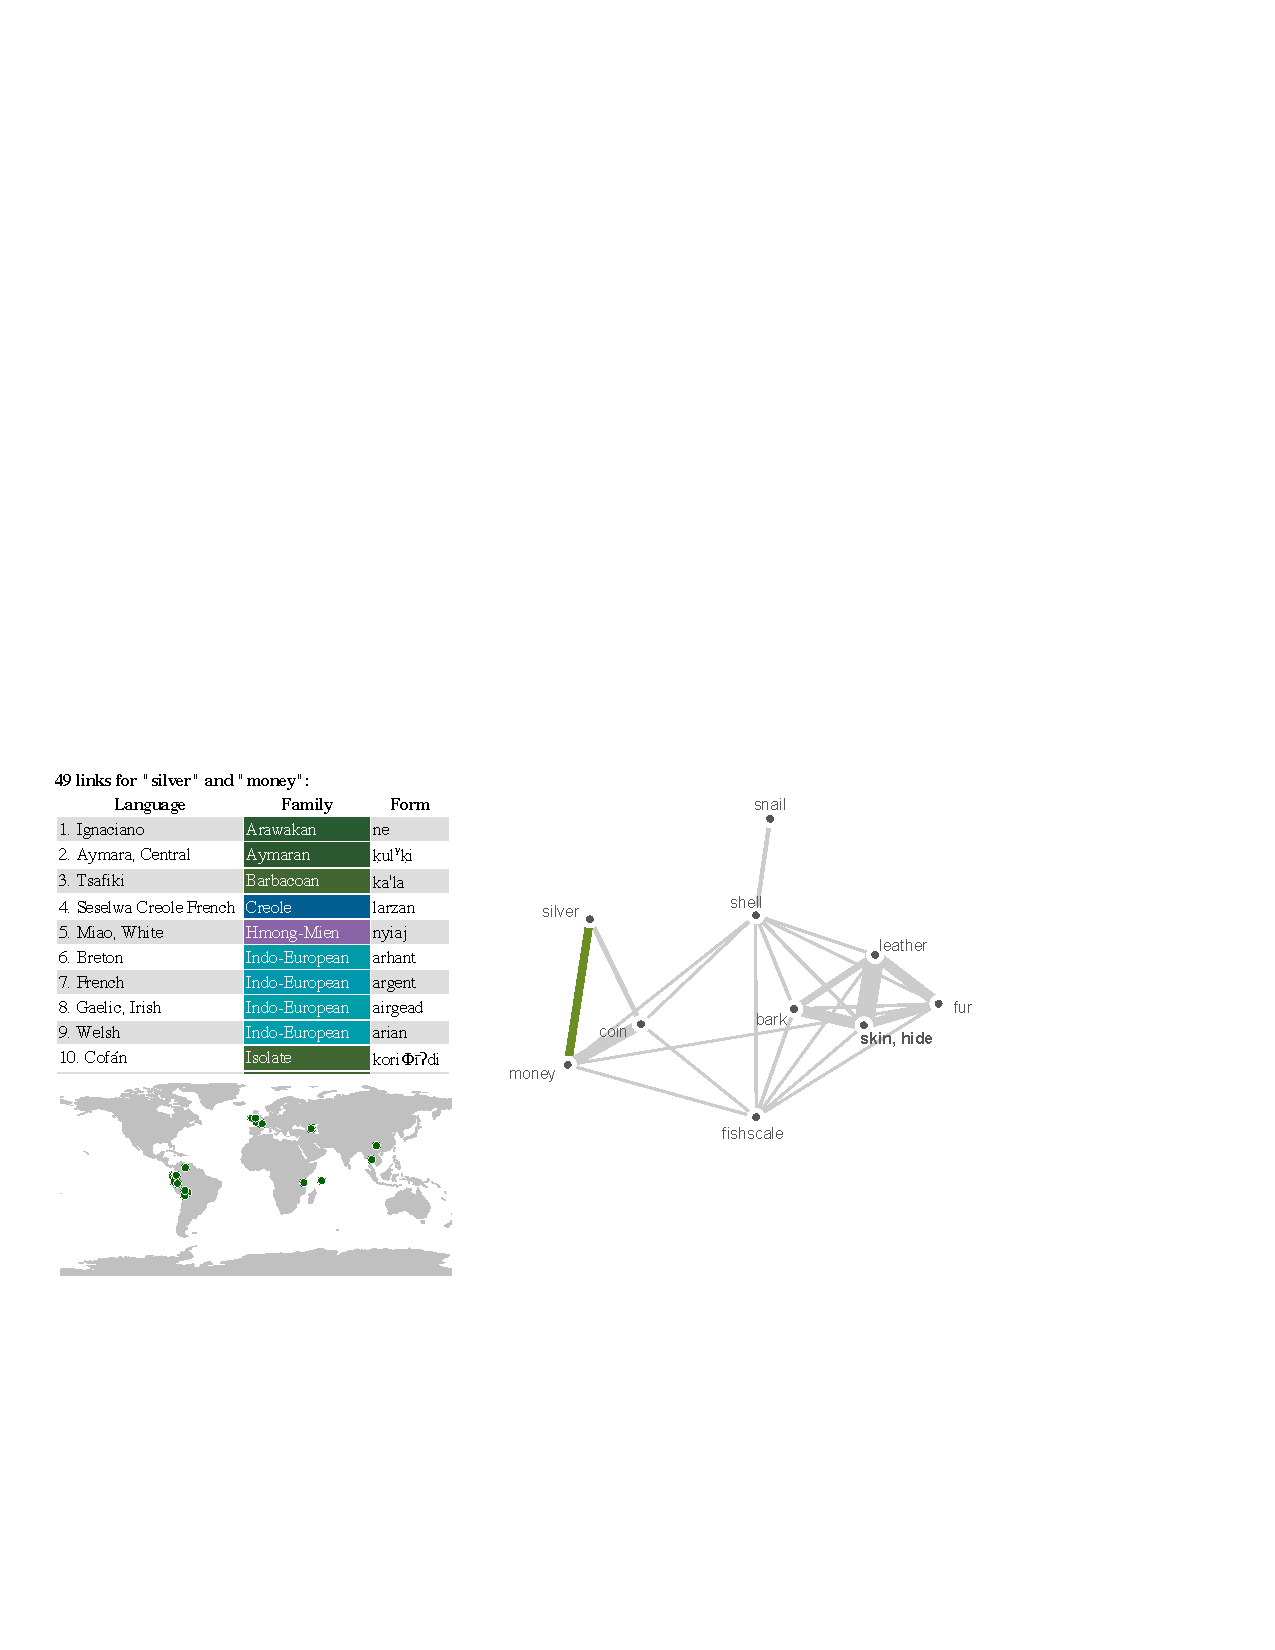
\includegraphics[width=12cm]{silvermoneyAREAL.pdf}}
\endpspicture}
\end{document}

